\documentclass[9pt]{beamer}

\usepackage{amsfonts}
\usepackage{amsmath}
\usepackage{amssymb}
\usepackage{cuted}
\usepackage{hyperref}
\usepackage{mathtools}
\usepackage{multirow}
\usepackage{siunitx}

\usetheme{Warsaw}

\AtBeginSection[]
{
    \begin{frame}
        \frametitle{Table of Contents}
        \tableofcontents[currentsection]
    \end{frame}
}

\title[Waveform and Passive Beamforming Design for IRS-Aided SWIPT]{Waveform and Passive Beamforming Design for Intelligent Reflecting Surface-Aided Wireless Information and Power Transfer}
\author{Yang Zhao}
\institute{Department of Electrical and Electronic Engineering\\ Imperial College London}
\date{Early Stage Assessment, \today}

\begin{document}

\frame{\titlepage}

\begin{section}{Introduction and Review}
	\begin{subsection}{From WPT to SWIPT}
		\begin{frame}{What is WPT?}
			\textbf{Wireless Power Transfer} (WPT) varies electromagnetic fields to deliver power.
			\begin{table}
				\scriptsize
				\caption{WPT Technologies}
				\begin{tabular}{|l|l|l|l|l|l|}
					\hline
					Categories                  & Technology                 & Devices           & Power                        & Frequency          & Range           \\ \hline
					\multirow{3}{*}{Near-field} & Magnetic resonant coupling & Resonators        & Up to 10 \si{\W}             & kHz -- MHz         & m               \\ \cline{2-6}
												& Inductive coupling         & Wire coils        & Up to 10 \si{\W}             & Hz -- MHz          & mm -- cm        \\ \cline{2-6}
												& Capacitive coupling        & Metal plates      & Up to 1 \si{\W}              & kHz -- MHz         & mm              \\ \hline
					\multirow{2}{*}{Far-field}  & \alert{RF waves}           & \alert{Rectennas} & \alert{\si{\uW} -- \si{\mW}} & \alert{MHz -- GHz} & \alert{m -- km} \\ \cline{2-6}
												& Light waves                & Lasers            & \si{\uW} -- \si{\mW}         & THz                & km              \\ \hline
				\end{tabular}
			\end{table}
		\end{frame}

		\begin{frame}{WPT by RF waves}
			\textbf{Energy flow}: DC $\to$ RF $\to$ RF $\to$ DC
			\begin{figure}
				\centering
				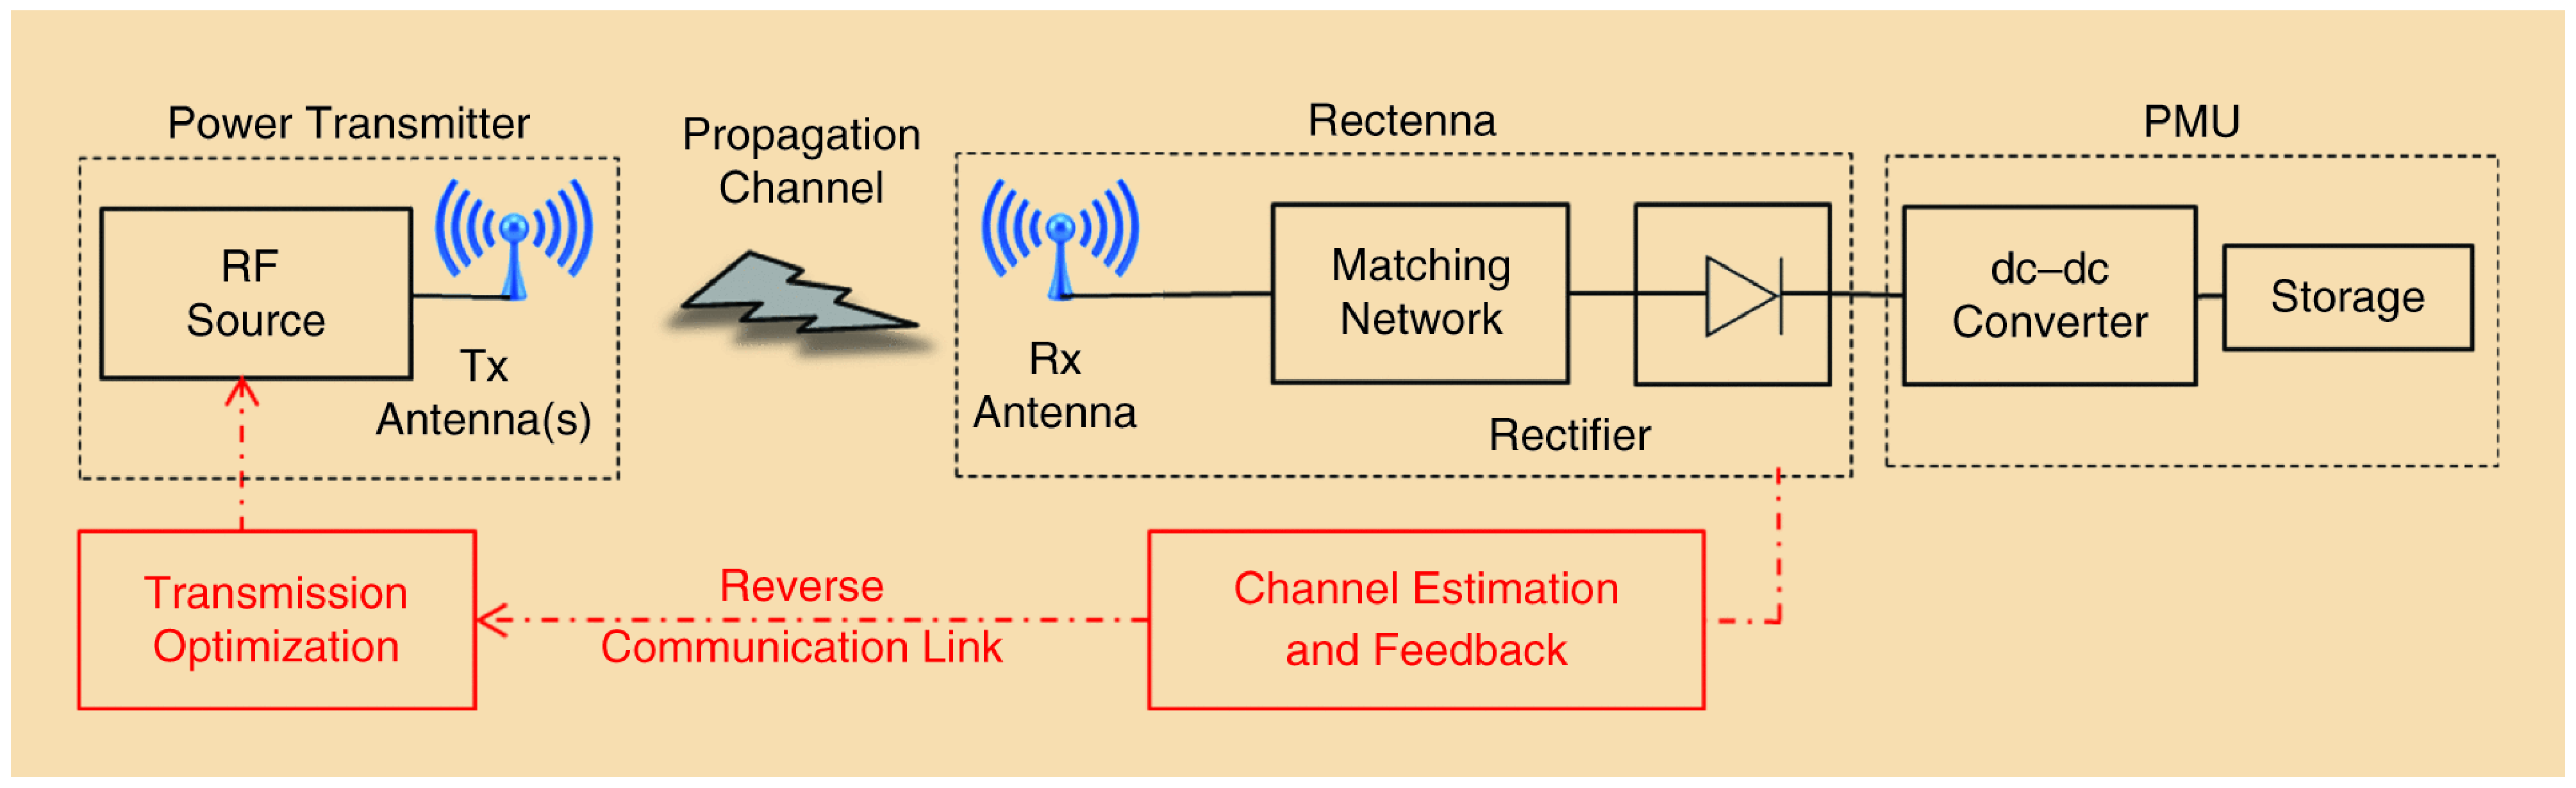
\includegraphics[width=\textwidth]{assets/wpt.eps}
			\end{figure}
			\textbf{Pros}:
			\begin{itemize}
				\item long range (up to hundreds of \si{\m}) with NLoS support
				\item compact receiver (few \si{\cm}), easy integration
				\item suitable for mobile devices
			\end{itemize}
			\textbf{Cons}:
			\begin{itemize}
				\item low power level (\si{\uW} -- \si{\mW})
				\item low energy harvesting efficiency (40\% at 100 \si{\uW}, 20\% at 10 \si{\uW})
			\end{itemize}
		\end{frame}
	\end{subsection}
\end{section}
\end{document}
